\chapter{绘制阀体立体图}

{\bfseries 学习目标}
\begin{itemize}
\item 学习利用chamfer命令绘制图形
\item 学习利用chamferedge命令建立三维倒角
\end{itemize}

{\bfseries 任务要求}
\begin{itemize}
\item 根据图\ref{fig:tiaoyafafati}所示的杯零件图,用旋转法建立调压阀阀体零件的三维模型
\end{itemize}

\noindent
\begin{figure}[htbp]
\centering
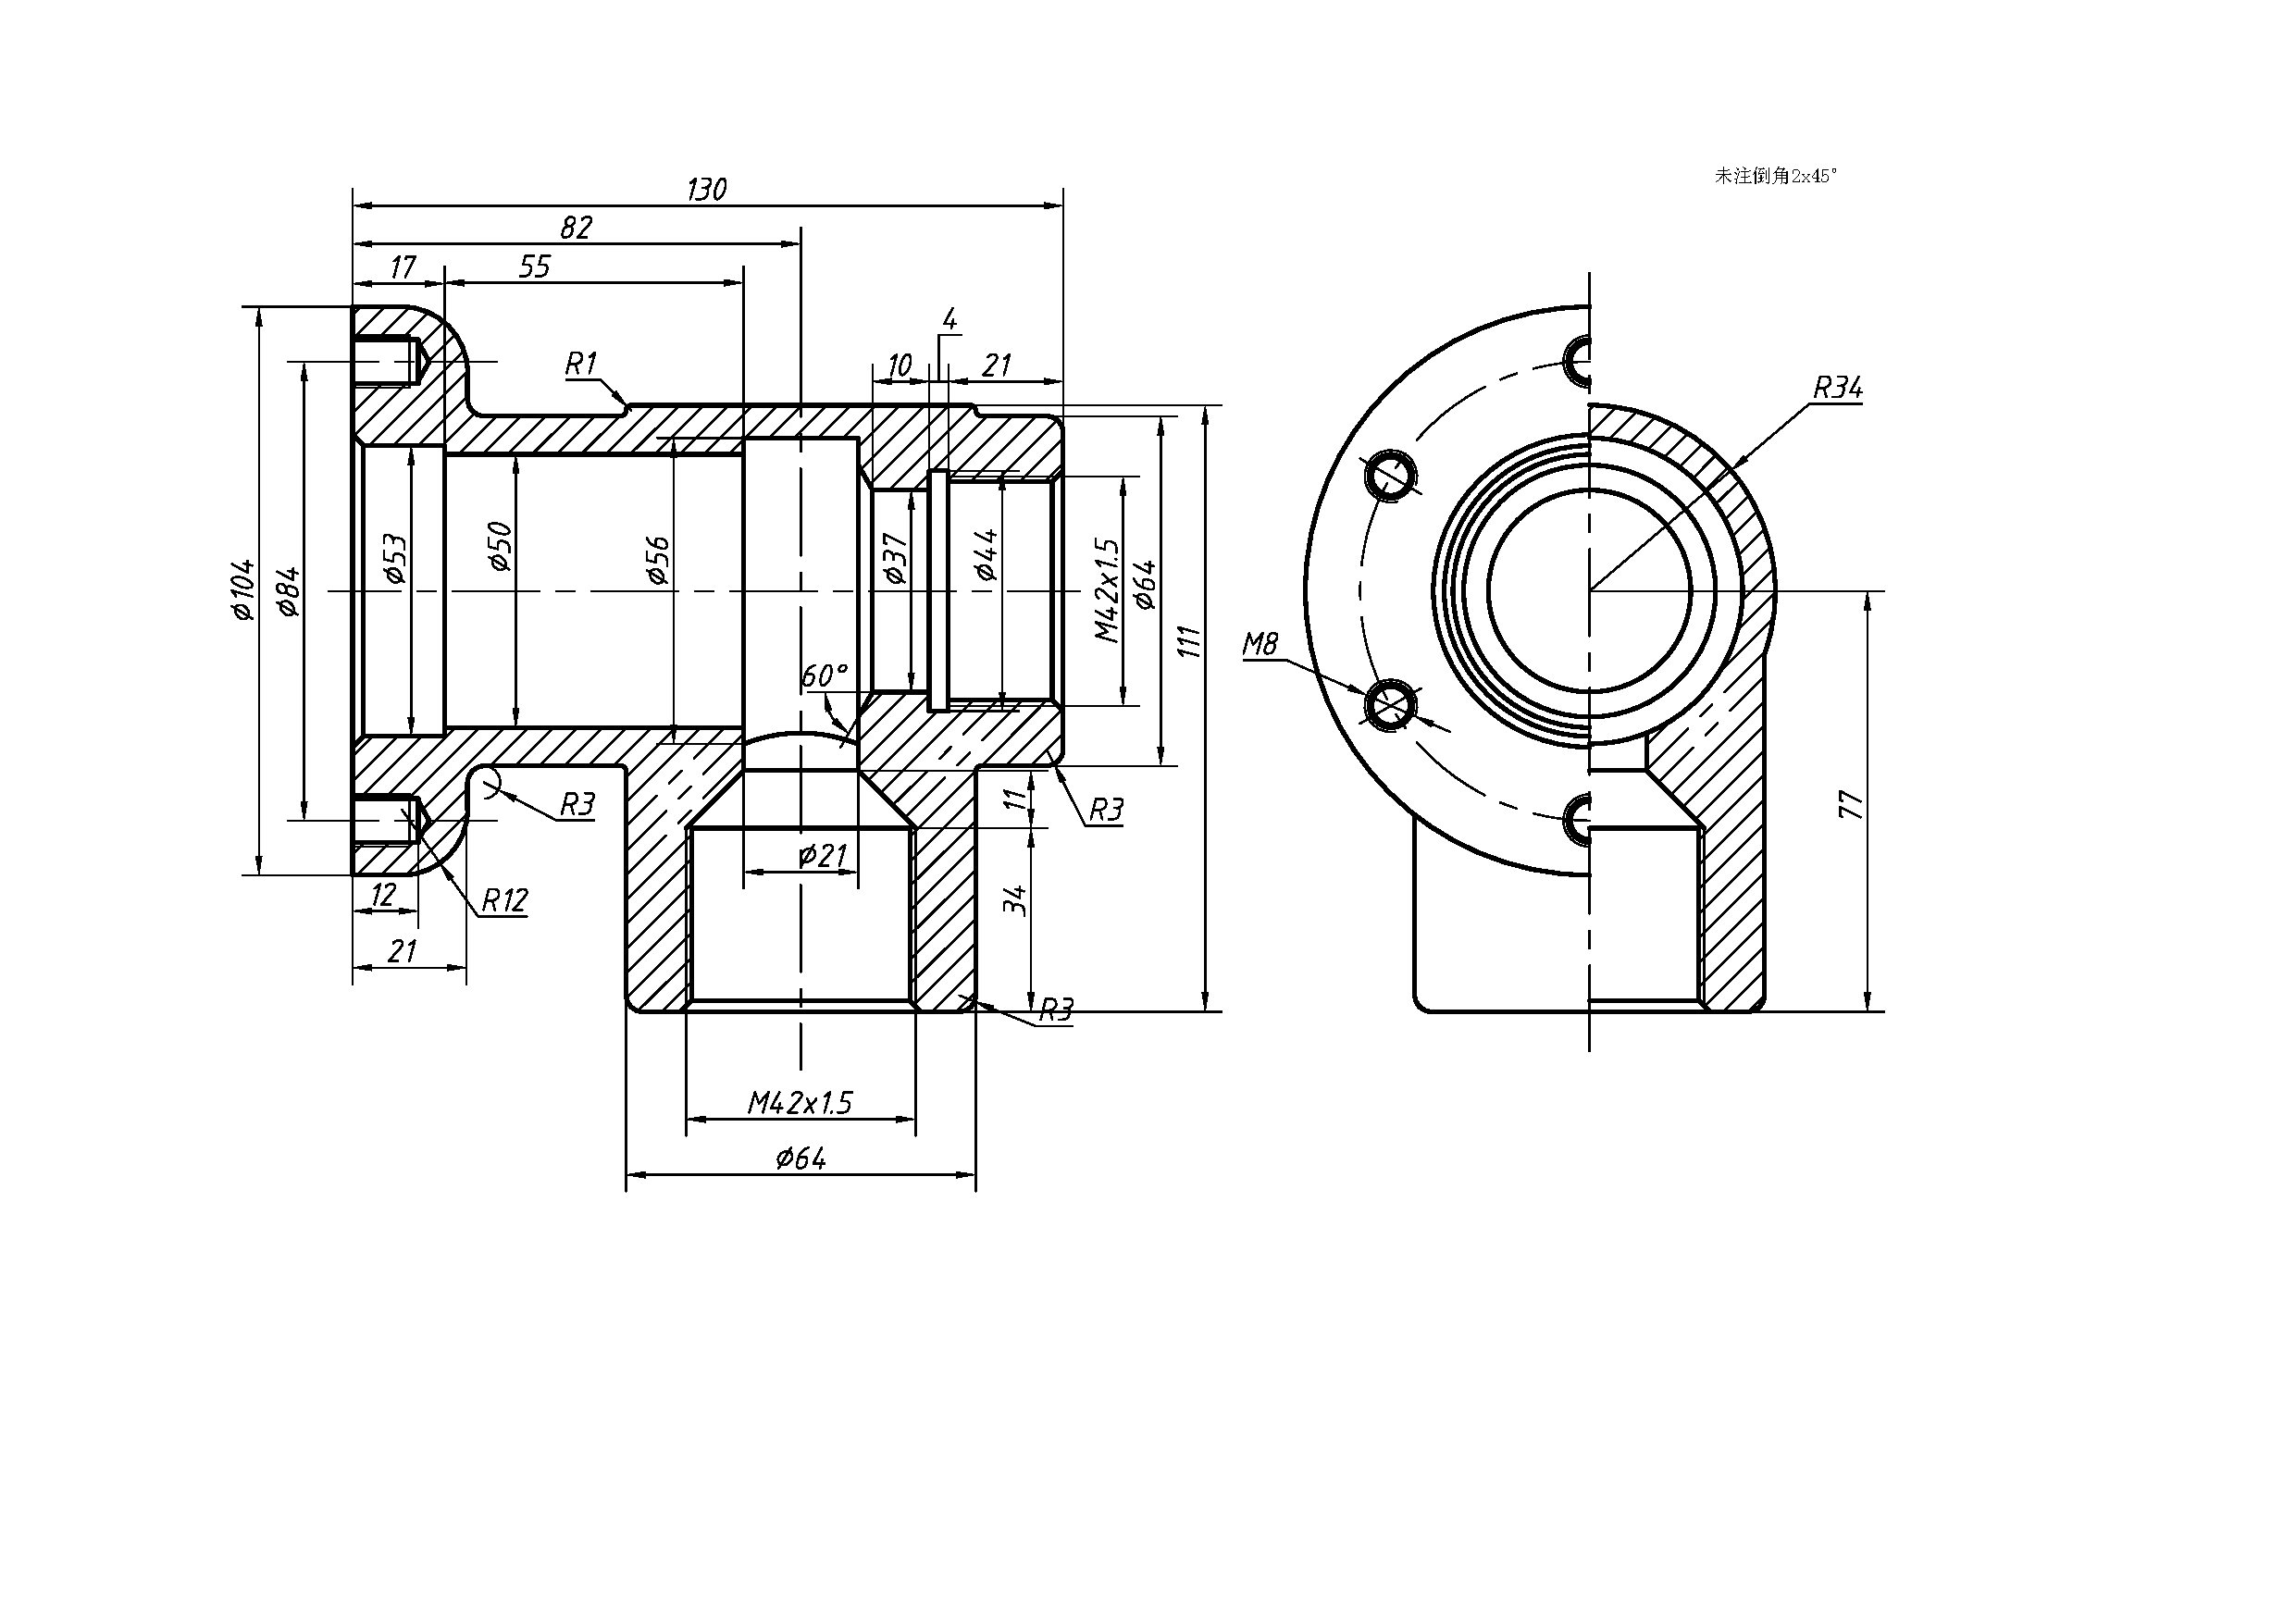
\includegraphics[scale=0.45]{tiaoyafafati.pdf}
\caption{阀体零件图}\label{fig:tiaoyafafati}
\end{figure}
\endinput